\section{Conclusioni}

\subsection{Correttezza}
La correttezza dell'implementazione di un test di ipotesi può essere controllata assicurandosi che in condizioni di ipotesi nulla il test produca esattamente $\alpha$\% falsi allarmi. Il test deve poi presentare la maggiore potenza possibile in caso di ipotesi contraria. Per utilizzare una metrica di riferimento abbiamo utilizzato i test inclusi nella libreria standard di matlab.
Mostriamo quindi il risultati ottenuti dall'uso di una semplice statistica, la differenza delle medie:

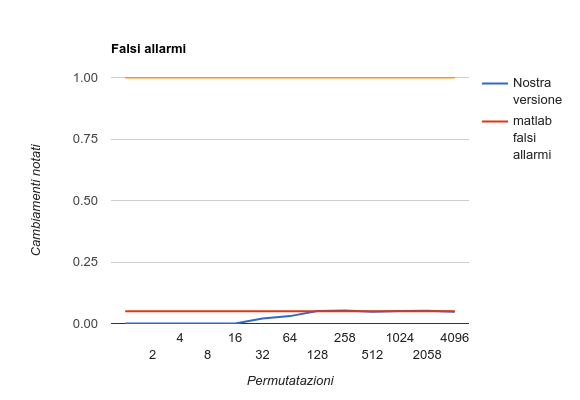
\includegraphics[width=\linewidth]{falsi_allarmi}

La linea rossa è generata da matlab non dipende dal numero di permutazioni, quindi è costante a 0.05, come ci si attende. La linea blu rappresenta invece la nostra versione del permutation test, la quale per bassi valori di permutazione è del tutto incapace di notare cambiamenti nei valori in ingresso. Quando le permutazioni aumentano i falsi allarmi si stabilizzano velocemente ad $\alpha$. 

Ora che siamo certi che sotto ipotesi nulla il nostro algoritmo si comporta correttamente, possiamo quindi analizzare il caso in cui i gruppi provengono da popolazioni diverse.

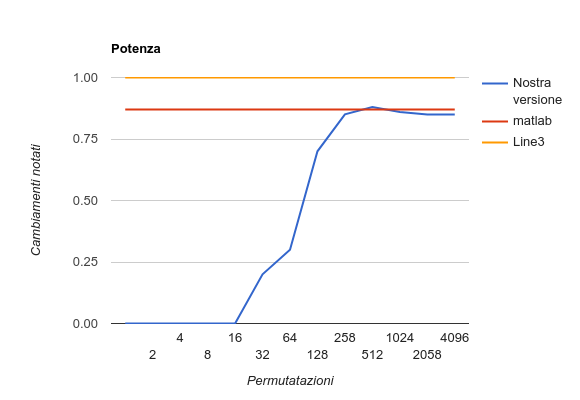
\includegraphics[width=\linewidth]{potenza}

Come nel caso precedente si nota che pur fallendo per permutazioni in quantità minute risulta che il test produce risultati simili a quello standard. Si noti inoltre che come nel caso precedente non sembra esserci alcun vantaggio nell'utilizzare una grandi numeri di permutazioni, poiché quando raggiungono l'ordine delle centinaia la potenza si stabilizza. Questo significa che, date le ottimizzazioni sull'uso della memoria, se si fissa un numero di permutazioni, è possibile processare set di dati con utilizzi di tempo e memoria che dipendono linearmente solo dalla dimensione dei dati in ingresso. Poiché è evidente che per processare un set di dati è per lo meno necessario valutare almeno una volta tutti gli elementi, ciò risulta essere il migliore risultato possibile. 

Ciò che rimane è mostrare la velocità di throughput che è possibile raggiungere è superiore ad un implementazione basata su cpu.

\subsection{Lavori Futuri}
A seconda di quale sia il campo di applicazione di un test di ipotesi ad alta performanza è possibile che ulteriori caratteristiche oltre a quelle indicare siano richieste. Si può immaginare che la necessità di analizzare eventi che avvengono ad alta frequenza sia spesso associata alla necessità di processare tali dati sotto forma di stream continui fino a che non viene notato un cambiamento nella natura dei dati osservati.
Una delle soluzioni di tale problema prende il nome di CPM e consiste nell'analizzare i dati una prima volta, per poi spostare il fucus dell'attenzione man mano che nuovi dati vengono ricevuti. Il tentativo di integrare efficientemente il permutation test e il cpm si è rivelato fallimentare. Inoltre, anche le integrazioni più semplici sono inefficienti, poiché le ottimizzazioni necessarie ad uno risultano deleterie all'altro. Questo limite pare significativo e ne consegue che la risoluzione possa essere soggetto di ulteriori studi.